\documentclass{article}
\usepackage{graphicx}
\usepackage{amsmath}
\usepackage{hyperref}

\title{Reporte del proyecto de Machine Learning}
\author{Alejandro Camacho C-412 \\ Ana Karla Caballero C-411}
\date{\today}

\begin{document}

\maketitle

\begin{abstract}
    En este proyecto, se propone un enfoque basado en aprendizaje automático para detectar el estado de deterioro de las calles en Cuba utilizando imágenes satelitales. Se utilizaron modelos preentrenados, que se especializan en segmentación semántica, para identificar y clasificar las diferentes condiciones de las calles. A través de un conjunto de datos de imágenes satelitales, se llevó a cabo un proceso de preprocesamiento y ajuste del modelo para optimizar su rendimiento en el contexto específico de Cuba. Los resultados indican una precisión notable en la detección de áreas deterioradas, lo que sugiere que esta metodología puede ser una herramienta valiosa para la gestión y planificación urbana en el país. Este trabajo destaca la importancia de la inteligencia artificial en la mejora de infraestructuras urbanas y proporciona una base para futuras investigaciones en la monitorización del estado de las calles a través de tecnologías de imágenes.
\end{abstract}

\section{Introducción}
El deterioro de las infraestructuras urbanas es un desafío crítico que afecta la calidad de vida de los ciudadanos y la eficiencia de los servicios públicos. En Cuba, donde las condiciones económicas y climáticas pueden agravar el estado de las calles, es fundamental implementar metodologías efectivas para monitorear y evaluar la infraestructura vial. Las calles deterioradas no solo representan un riesgo para la seguridad de los transeúntes, sino que también impactan en la movilidad y el acceso a servicios básicos.

En la última década, el uso de imágenes satelitales ha demostrado ser una herramienta poderosa para la observación y análisis de fenómenos geoespaciales. Estas imágenes permiten una cobertura extensa y la recopilación de datos en tiempo real, lo que resulta esencial para la planificación urbana y la gestión de infraestructuras. Sin embargo, el análisis manual de estas imágenes es laborioso y propenso a errores, lo que ha llevado al interés en el uso de técnicas de aprendizaje automático para automatizar este proceso.

El objetivo de este proyecto es desarrollar un enfoque automatizado que permita identificar y clasificar las condiciones de las calles, proporcionando información valiosa para la toma de decisiones en la gestión urbana. A través de la implementación de este modelo, se espera contribuir al desarrollo de soluciones tecnológicas que mejoren la sostenibilidad y la eficiencia de las infraestructuras en Cuba.

En este informe, se presentará una revisión de la literatura relacionada, seguida de una descripción detallada de la metodología utilizada, los resultados obtenidos y una discusión sobre las implicaciones de los hallazgos. Finalmente, se ofrecerán conclusiones y recomendaciones para futuras investigaciones en el área.

\section{Estado del Arte}

\subsection{Evoluci\'on de las Redes Neuronales Convolucionales (CNN)}
La segmentación semántica es una técnica crucial en el campo de la visión por computadora que permite asignar una etiqueta a cada píxel de una imagen. Esta técnica ha evolucionado significativamente desde sus inicios en la década de 2000, impulsada por avances en algoritmos de aprendizaje profundo y arquitecturas de redes neuronales.

\subsubsection{Redes Neuronales Convolucionales (CNN)}
Las CNN \href{https://www.semanticscholar.org/paper/Rich-Feature-Hierarchies-for-Accurate-Object-and-Girshick-Donahue/2f4df08d9072fc2ac181b7fced6a245315ce05c8}{1} fueron uno de los primeros enfoques exitosos para la segmentación semántica. Estas redes utilizan capas convolucionales para extraer características relevantes de las imágenes.

\subsubsection{Fully Convolutional Networks (FCN) \href{https://www.semanticscholar.org/paper/Fully-convolutional-networks-for-semantic-Shelhamer-Long/6fc6803df5f9ae505cae5b2f178ade4062c768d0}{2}} 
En 2015, se introdujeron las redes completamente convolucionales (FCN), que reemplazan las capas densas por capas convolucionales, permitiendo una mejor preservación de la resolución espacial. Este enfoque facilitó la segmentación a nivel de píxel y mejoró significativamente la precisión en tareas complejas.

\subsubsection{DeepLab}
Desarrollado por Google, DeepLab\href{https://www.semanticscholar.org/paper/DeepLab%3A-Semantic-Image-Segmentation-with-Deep-and-Chen-Papandreou/cab372bc3824780cce20d9dd1c22d4df39ed081a}{3} utiliza convoluciones dilatadas para aumentar el campo receptivo sin perder resolución espacial. Esta arquitectura ha demostrado ser efectiva en múltiples benchmarks y es utilizada en aplicaciones como la segmentación semántica de imágenes satelitales.


La segmentación semántica se ha aplicado con éxito para evaluar el estado del deterioro de infraestructuras urbanas. En particular, el uso de imágenes satelitales permite una evaluación a gran escala y con alta precisión. Modelos como FCN ResNet50 han sido utilizados para clasificar diferentes estados del pavimento y detectar áreas críticas que requieren atención \href{https://www.semanticscholar.org/paper/Semantic-Segmentation-of-Urban-Street-Scenes-Using-Noori-Shaker/a86227d6ffaa1cad529a78b66faf8bdb57f4fb16}{4}.

\subsection{Aplicaciones de Imágenes Satelitales en Análisis Urbano}
\begin{enumerate}
    \item Las imágenes satelitales se utilizan para monitorear el crecimiento urbano y los cambios en el uso del suelo. Por ejemplo, el proyecto titulado"Comparative Analysis of Different CNN Models for Semantic Segmentation" de Sariturk y Kumbasar se centra en la evaluación comparativa de diversas arquitecturas de redes neuronales convolucionales (CNN) para la segmentación semántica. El estudio investiga cómo diferentes modelos de CNN, como U-Net, FCN y DeepLab, se desempeñan en tareas de segmentación semántica, analizando su precisión y eficiencia en el procesamiento de imágenes.

    Este análisis proporciona información valiosa sobre la selección de modelos para tareas específicas de segmentación semántica, lo que puede ser relevante para proyectos similares que buscan optimizar el rendimiento en la clasificación de imágenes. \href{https://www.semanticscholar.org/paper/Comparative-Analysis-of-Different-CNN-Models-for-Sariturk-Kumbasar/d8400a08b6e0a6bd74ec80e5cfd3295659222b90}{5}
    
    \item El artículo titulado "Objective scoring of streetscape walkability to evaluate urban environments" de Nagata y Nakaya se centra en la evaluación objetiva de la caminabilidad de las calles urbanas. Los autores proponen un enfoque sistemático para medir la calidad del entorno urbano en términos de su accesibilidad y comodidad para los peatones.

    Este enfoque no solo proporciona una herramienta útil para planificadores urbanos y arquitectos, sino que también contribuye a la promoción de entornos más amigables para los peatones, lo que es fundamental para el desarrollo sostenible de las ciudades. La metodología presentada puede ser relevante para proyectos que buscan evaluar y mejorar la infraestructura urbana, como el análisis del estado de deterioro de calles. \href{https://www.semanticscholar.org/paper/Objective-scoring-of-streetscape-walkability-to-of-Nagata-Nakaya/3ab9cb125263f3aee87237be3fc037f916e38275}{6}
    
    \item Mapillary es una plataforma colaborativa que permite la captura y el intercambio de imágenes de nivel de calle, geolocalizadas, con el objetivo de mejorar la cartografía y la representación del entorno urbano. Esta utiliza tecnologías de visión por computadora y Big Data para procesar estas imágenes, facilitando así la actualización y mejora de mapas en tiempo real.
    
    Mapillary es especialmente útil porque proporciona un acceso a una amplia variedad de imágenes urbanas que pueden complementar los datos obtenidos a través de imágenes satelitales. Esto permite una evaluación más precisa del estado de deterioro de las calles, ya que las imágenes capturadas a nivel del suelo pueden ofrecer información detallada sobre las condiciones específicas de las infraestructuras. \href{https://www.mapillary.com/}{7}
\end{enumerate}

\subsection{Retos}
A pesar del avance en el uso de imágenes satelitales, el proyecto realizado se enfrent\'o a varios retos en su creación:

\subsubsection{Tama\~no del dataset}
No se pudo encontrar un dataset acorde a nuestro problema por lo que se tuvo que crear uno utilizando distintas t\'ecnicas de aumentaci\'on de datos.

\subsubsection{Variabilidad en las Condiciones de Iluminación}
Las condiciones de iluminación pueden variar significativamente entre las imágenes adquiridas, afectando la consistencia y precisión del análisis. Esto es especialmente relevante en áreas urbanas donde las sombras proyectadas por edificios pueden alterar los datos espectrales.

\subsubsection{Condiciones Climáticas}
Las condiciones climáticas también pueden influir en la calidad de las imágenes satelitales. Factores como nubes, lluvia o neblina pueden obstruir las vistas y afectar los datos obtenidos, complicando el análisis posterior.

\subsubsection{Resolución de las Imágenes}
La resolución espacial de las imágenes es un factor crítico. Imágenes con baja resolución pueden no capturar detalles necesarios para una segmentación precisa, mientras que imágenes de alta resolución pueden ser costosas y difíciles de obtener.


\section{Metodología}
Dado que el presente proyecto tiene como objetivo principal evaluar el estado de deterioro de las calles mediante el análisis de imágenes satelitales, se implementan dos arquitecturas de redes neuronales avanzadas: **FCN ResNet50** y **DeepLab**. La elección de estos modelos se fundamenta en su capacidad para realizar segmentación semántica, lo que permite identificar con precisión las áreas afectadas por el deterioro.

A través de la comparación del rendimiento de ambos modelos, se busca no solo determinar cuál ofrece una mayor precisión en la clasificación del estado de las calles, sino también comprender mejor las características que influyen en su efectividad.

\subsection{Datos}
La creación de la base de datos representó un desafío significativo durante la implementación del proyecto, dado que la evaluación del estado de una calle a partir de imágenes satelitales es una tarea compleja que resulta difícil de realizar a simple vista. Se llevó a cabo una búsqueda exhaustiva en diversas plataformas y aplicaciones, incluidas Kaggle, Mapillary y Google Maps, donde se lograron recopilar un total de 37 imágenes satelitales provenientes de diferentes áreas de La Habana.

Dado que la cantidad de datos recolectados no constituía un número suficiente para llevar a cabo una investigación robusta, se implementaron diversas técnicas de aumento de datos, tales como rotación y volteo. Estas técnicas permitieron expandir el conjunto de datos hasta alcanzar un total de 108 imágenes, de las cuales 88 fueron asignadas para el entrenamiento y 20 para la validación del modelo.

Posteriormente, se utilizó la herramienta Labelme para crear máscaras que señalaran las condiciones de las calles, clasificándolas en buen estado y mal estado. Este proceso fue laborioso y ralentizó el avance del proyecto, ya que tuvo que realizarse manualmente.

\subsection{Algoritmos y Resultados obtenidos}
\section{Metodología}
La metodología del proyecto se centra en la utilización de modelos de aprendizaje profundo, específicamente el modelo preentrenado DeepLabv3, para evaluar el estado de deterioro de las calles de Cuba a partir de imágenes satelitales. A continuación se detalla el proceso seguido en cada fase del entrenamiento.

\subsection{Entrenamiento Inicial}
En la primera fase, se llevó a cabo un entrenamiento inicial del modelo DeepLabv3. Durante este proceso, se observó que la reducción en la calidad de las imágenes resultó en una pérdida significativa de información, lo que afectó negativamente los resultados. Los modelos entrenados en esta etapa mostraron un rendimiento insatisfactorio, con una detección deficiente del estado de las calles.


\begin{figure}
    \centering
    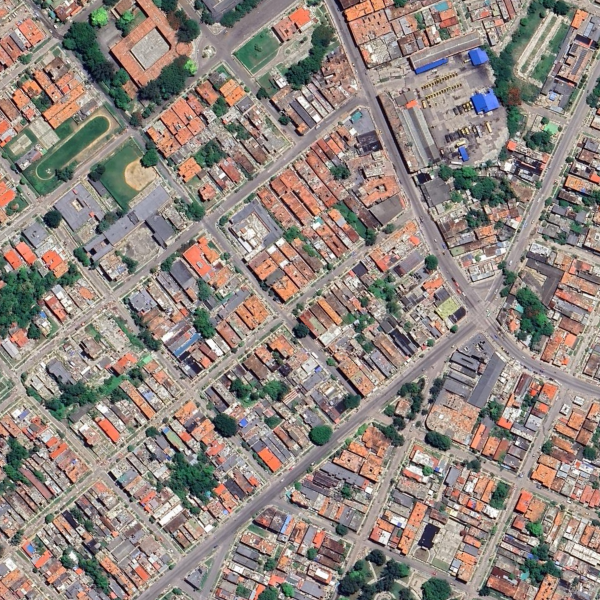
\includegraphics[width=0.5\textwidth]{/media/roxy/829A20F39A20E4FF/new/Road-Pothole-Detection-main/predicted/model_deeplabv3_resnet101_ts256,256_bs5_ep30.pth/7.png} % Adjust width as needed
    \caption{Input} % Image caption
    \label{fig:input} % Label for cross-references
\end{figure}

\begin{figure}
    \centering
    \includegraphics[width=0.5\textwidth]{/media/roxy/829A20F39A20E4FF/new/Road-Pothole-Detection-main/predicted/model_deeplabv3_resnet101_ts256,256_bs5_ep30.pth/7 prediction.png} % Adjust width as needed
    \caption{Output Model 1} % Image caption
    \label{fig:input} % Label for cross-references
\end{figure}

\begin{figure} 
    \centering
    \includegraphics[width=0.8\textwidth]{/media/roxy/829A20F39A20E4FF/new/Road-Pothole-Detection-main/predicted/model_deeplabv3_resnet101_ts256,256_bs5_ep30.pth/7_confusion_matrix.png} % Adjust width as needed
    \caption{Matriz de confusión Model 1} % Image caption
    \label{fig:matriz_confusion} % Label for cross-references
\end{figure}

\subsection{Mejoras en el Entrenamiento}
Con base en los resultados obtenidos en la primera fase, se implementaron mejoras significativas en el segundo intento de entrenamiento. Se utilizó el conjunto de imágenes sin restarle calidad y se ajustaron parámetros clave del modelo: el peso. En esta fase, el modelo mostró una mejora notable en la detección de las condiciones de las calles, logrando identificar con mayor precisión las áreas en mal estado y aquellas que estaban en buen estado.

\begin{figure}
    \centering
    \includegraphics[width=0.5\textwidth]{/media/roxy/829A20F39A20E4FF/new/Road-Pothole-Detection-main/predicted/model_deeplabv3_resnet101_ts300,300_bs2_ep4_w.pth/7 prediction.png} % Adjust width as needed
    \caption{Output Model 2} % Image caption
    \label{fig:input} % Label for cross-references
\end{figure}

\begin{figure} 
    \centering
    \includegraphics[width=0.8\textwidth]{/media/roxy/829A20F39A20E4FF/new/Road-Pothole-Detection-main/predicted/model_deeplabv3_resnet101_ts300,300_bs2_ep4_w.pth/7_confusion_matrix.png} % Adjust width as needed
    \caption{Matriz de confusión Model 2} % Image caption
    \label{fig:matriz_confusion} % Label for cross-references
\end{figure}


\subsection{Aumento de Épocas y Resultados Finales}
Uno de los cambios más relevantes fue el aumento del número de épocas durante el entrenamiento a 100. Este ajuste permitió al modelo aprender patrones más complejos y mejorar su capacidad para clasificar el estado de deterioro de las calles. Los resultados obtenidos fueron significativamente mejores en comparación con los entrenamientos anteriores, evidenciando un avance considerable en la detección.

\begin{figure}
    \centering
    \includegraphics[width=0.5\textwidth]{/media/roxy/829A20F39A20E4FF/new/Road-Pothole-Detection-main/predicted/model_deeplabv3_resnet101_ts315,315_bs4_ep10_w.pth/7 prediction.png} % Adjust width as needed
    \caption{Output Model 3} % Image caption
    \label{fig:input} % Label for cross-references
\end{figure}

\begin{figure} 
    \centering
    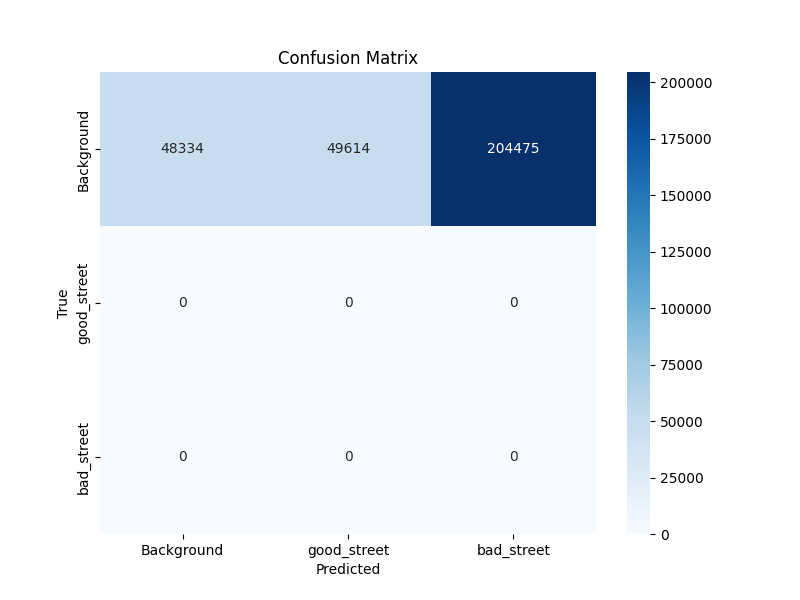
\includegraphics[width=0.8\textwidth]{/media/roxy/829A20F39A20E4FF/new/Road-Pothole-Detection-main/predicted/model_deeplabv3_resnet101_ts315,315_bs4_ep10_w.pth/12_confusion_matrix.png} % Adjust width as needed
    \caption{Matriz de confusión Model 3} % Image caption
    \label{fig:matriz_confusion} % Label for cross-references
\end{figure}

\section{Conclusiones}
A pesar de los avances logrados, se identificó que un conjunto de datos más amplio y diverso podría haber mejorado aún más la precisión del modelo. La falta de datos adecuados limita la capacidad del modelo para generalizar y ofrecer resultados más precisos. Para futuras investigaciones, se recomienda la recopilación y etiquetado de un conjunto de datos más extenso que incluya diversas condiciones y tipos de deterioro.

\section*{Referencias}
\begin{enumerate}
    \item https://www.semanticscholar.org/paper/Rich-Feature-Hierarchies-for-Accurate-Object-and-Girshick-Donahue/2f4df08d9072fc2ac181b7fced6a245315ce05c8
    \item https://www.semanticscholar.org/paper/Fully-convolutional-networks-for-semantic-Shelhamer-Long/6fc6803df5f9ae505cae5b2f178ade4062c768d0
    \item https://www.semanticscholar.org/paper/DeepLab%3A-Semantic-Image-Segmentation-with-Deep-and-Chen-Papandreou/cab372bc3824780cce20d9dd1c22d4df39ed081a
    \item https://www.semanticscholar.org/paper/Semantic-Segmentation-of-Urban-Street-Scenes-Using-Noori-Shaker/a86227d6ffaa1cad529a78b66faf8bdb57f4fb16\
    \item https://www.semanticscholar.org/paper/Comparative-Analysis-of-Different-CNN-Models-for-Sariturk-Kumbasar/d8400a08b6e0a6bd74ec80e5cfd3295659222b90
    \item https://www.semanticscholar.org/paper/Objective-scoring-of-streetscape-walkability-to-of-Nagata-Nakaya/3ab9cb125263f3aee87237be3fc037f916e38275
    \item https://www.mapillary.com/
\end{enumerate}

\end{document}